\documentclass[12pt,includeheadfoot,a4paper]{report}
\usepackage[print,nopanel]{pdfscreen}
%\begin{print}
\usepackage{lipsum}% http://ctan.org/pkg/lipsum
\usepackage{titletoc}
%\section{type}
\usepackage{lastpage}
\usepackage{macro/macro}
\usepackage{float}
\usepackage{fancyhdr}
\usepackage{booktabs}
\usepackage{array}
\newcolumntype{K}[1]{>{\centering\arraybackslash}p{#1}}
\usepackage{xcolor, colortbl}
\definecolor{Gray}{gray}{0.85}
\usepackage{verbatim}
\usepackage[Glenn]{fncychap}
\usepackage{placeins}
\let\Oldsubsection\subsection
\renewcommand{\subsection}{\FloatBarrier\Oldsubsection}
\lhead{\bfseries OpenSCAD's customizer}
\rhead{}
\usepackage[left=2.5cm, right=1.5cm, top=1.5cm, bottom=1.5cm]{geometry}
\pagestyle{fancy}
%\end{print}
\margins{2.5cm}{1.5cm}{1.5cm}{1.5cm}
\linespread{1.25}
\screensize{8cm}{9cm}
\overlay{overlay8.pdf}
\usepackage{graphicx}


\begin{document}
	\newcommand{\centertext}[1]{\begin{center}\textbf{#1}\end{center}}
\newcommand{\student}{\vskip 2.5cm}
\newcommand{\supervisor}{\vskip 2cm}
\newcommand{\stamp}{\vskip 2.5cm}
\newcommand{\HRule}{\rule{\linewidth}{0.5mm}}
\newcommand{\projecttitle}{ \fontsize{24}{25}\selectfont \bf{OpenSCAD's Customizer}}
\newcommand{\tab}[1]{\hspace{.4\textwidth}\rlap{#1}}
\newcommand{\itab}[1]{\hspace{.05\textwidth}\rlap{#1}}
\newcommand{\logo}[1]{\includegraphics[scale=0.16]{#1}}
\newcommand{\submitted}{
\vskip 0.4in
\textnormal{ {\fontsize{14}{16}\selectfont \textbf{Project Synopsis}} \\
	{\fontsize{12}{13}\selectfont of Major Project}\\
}
\vskip 0.2in

\textnormal{
 {\fontsize{14}{16}\selectfont \textbf{Bachelor of Technology}\\}
 {\fontsize{16}{17}\selectfont  (Computer Science and Engineering)\\}
}
\vskip 2cm
%\image{0.7}{images/gne.png}{}

\includegraphics[width=7cm]{images/gne.png}
\vskip 2cm
\begin{minipage}{0.4\textwidth}
\begin{flushleft} \large
{Submitted by:}\\
\textnormal{{\fontsize{12}{13}\selectfont Amarjeet Singh Kapoor\\ D4CSE 2013-17 \\135005\\1311017 \\}} % Your name
\end{flushleft}
\end{minipage}
~
\begin{minipage}{0.4\textwidth}
\begin{flushright}
\textnormal{ \\
	 {\fontsize{12}{13}\selectfont B-33, 1912, Bhagwna dass colony\\ Ludhiana\\
	9417321813\\ amarjeet.kapoor1@gmail.com \\                                                                                     }} % Supervisor's Name
\end{flushright}
\end{minipage}\\[1.5cm]
\HRule \\[0.4cm]

\textnormal{
Guru Nanak Dev Engineering College \\
Ludhiana 141006}
}


\newcommand{\pagetitle}{\begin{center}
\projecttitle
\Large\textbf{}\\
\submitted
\vskip 1cm

\end{center}}
\newcommand{\openoffice}{\textbf{OpenOffice}}
\newcommand{\frontmatter}[1]{\begin{Large} \textbf{#1} \end{Large}}
\newcommand{\ppttitle}{\begin{center}
\end{center}}

	\begin{screen}
		\ppttitle
	\end{screen}
\thispagestyle{empty} 
\pagetitle
\newpage
\pagenumbering{Roman}
\cfoot{\thepage}

\begin{Large}
\centertext{Abstract}
\end{Large}


User Interface for Customizing Models in OpenSCAD is the project that I worked upon for my 6-month training and also as Google summer of code project. It is under the umbrella organization of BRL-CAD. OpenSCAD is an open source organization that serves a free software to create solid 3d CAD objects. OpenSCAD has in a way redefined how easy 3D modeling can be. But the Wikipedia article on OpenSCAD says that it is a non-interactive modeler, but rather a 3D compiler based on a textual description language. Pay attention to the above line, it’s primarily what I’ll be talking about.

What the guys over at Wikipedia said is true but their version of the truth needs a little filtration (rather trimming). OpenSCAD’s way of customization is interactive, just not through a graphical interface. And this contingency makes the whole 3D modeling thing a little less easy than it can be. But all of that is about to change.

Solid 3D modeling. That sounds like some serious business. But it’s just an awesome tool for making models pertaining to many uses (mostly 3D printing). And 3D printing as we can all agree upon is cool. 3D models can be created by anyone using OpenSCAD. OpenSCAD is as much for designers as it is for you and me. What else can most people agree upon apart from the fact that solid 3D modeling is cool? A graphical interface is simpler and more intuitive to use. There is a general aversion for typing commands in order to get things done. Simply put, more people have an inclination towards GUI.

This is something that OpenSCAD lacked. But the benevolent folks at Thingiverse.com found a way to help out the demographic intersection of GUI lovers and OpenSCAD users. The website provides an easy to use interface to customize models of OpenSCAD. All one needs to do is upload the OpenSCAD file. After uploading the file, what you’ll see can only be described as being magic. I’m kidding, it’s just very useful is all. The OpenSCAD’s script is used to make a form containing slide bars, text boxes, combo boxes, labels, etc all for the singular purpose of customizing models.

My project was to include similar functionality into OpenSCAD itself. Constantly having to upload files created in one software (OpenSCAD) to a website in order to customize your models can get a little problematic as one is uploading scripts without being able to confirm how the script will translate into a form on the site. Wouldn’t it be great if everything is at one place, the original place: OpenSCAD? Of course, it would.

My project intends to define a user interface to customize models interactively instead of having to modify them manually. It will enable the user to create the templates for a given model which can further be changed as per user’s requirements.

This project will allow the modelers to create generic models (templates) which others can then customize to cater to their own use.
\newpage
\begin{Large}
\centertext{Acknowledgement}
\end{Large}

I, student of Guru Nanak Dev Engineering College, Ludhiana, have taken efforts in this project.
However, it would not have been possible without the kind support and help of many individuals
and organizations. I would like to extend my sincere thanks to all of them.\\

The author is highly grateful to Dr. M.S. Saini Director, Guru Nanak Dev Engineering College, Ludhiana for providing him with the opportunity to carry out his Six Weeks Training at
Testing and Consultancy Cell, Guru Nanak Dev Engineering College, Ludhiana.\\

The author would like to whole heartedly thank Dr. H.S. Rai Dean, Testing and Consultancy
Cell, Guru Nanak Dev Engineering College, Ludhiana who is a vast sea of knowledge and without whose constant and never ending support and motivation, it would never have been possible to complete the project and other assignments so efficiently and effectively.\\

Finally, I would thanks My Mentors at OpenSCAD organisation Marius Kintel and Torsten Paul. Without their encouragementand Guidence it would not have been possible to complete this project
in such an efficient manner.


\vskip 1.0cm 
\noindent Amarjeet Singh Kapoor


\tableofcontents
\listoffigures
\pagenumbering{arabic}
\cfoot{\thepage}

\chapter{INTRODUCTION}
\section{Overview}
\begin{figure}[H] 
	\centering 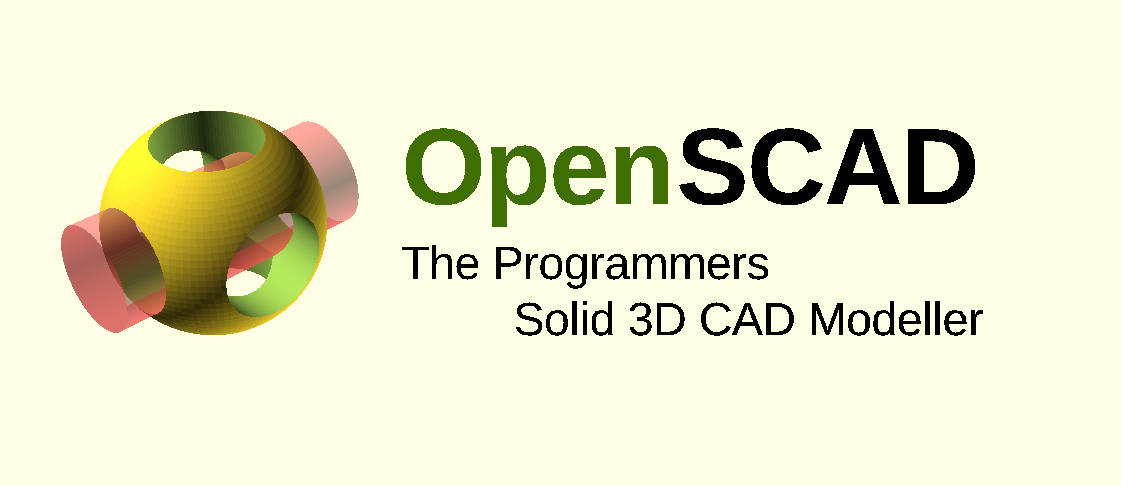
\includegraphics[scale=0.31]{images/openscad.png}
	\caption{OpenSCAD's logo}
	\label{fig:openscadlogo}
\end{figure}

User Interface for Customizing Models in OpenSCAD is the project that I worked upon for my 6-month training. It is under the umbrella organization of BRL-CAD. OpenSCAD is a free and Open-source software application for creating solid 3D CAD objects. It is a script only based modeler, with a specific description language. Parts cannot be selected or modified by mouse in the 3D view. An OpenSCAD script specifies geometric primitives and defines how they are modified and manipulated to render a 3D model. OpenSCAD is available for Windows, Linux and OS X. It does constructive solid geometry (CSG).

OpenSCAD has in a way redefined how easy 3D modeling can be. But the Wikipedia article on OpenSCAD says that it is a non-interactive modeler, but rather a 3D compiler based on a textual description language. Pay attention to the above line, it’s primarily what I’ll be talking about.

Solid 3D modeling. That sounds like some serious business. But it’s just an awesome tool for making models pertaining to many uses (mostly 3D printing). And 3D printing as we can all agree upon is cool. 3D models can be created by anyone using OpenSCAD. OpenSCAD is as much for designers as it is for you and me. What else can most people agree upon apart from the fact that solid 3D modeling is cool? A graphical interface is simpler and more intuitive to use. There is a general aversion for typing commands in order to get things done. Simply put, more people have an inclination towards GUI.

This is something that OpenSCAD lacked. But the benevolent folks at Thingiverse.com found a way to help out the demographic intersection of GUI lovers and OpenSCAD users. The website provides an easy to use interface to customize models of OpenSCAD. All one needs to do is upload the OpenSCAD file. After uploading the file, what you’ll see can only be described as being magic. I’m kidding, it’s just very useful is all. The OpenSCAD’s script is used to make a form containing slide bars, text boxes, combo boxes, labels, etc all for the singular purpose of customizing models.

My project was to include similar functionality into OpenSCAD itself. Constantly having to upload files created in one software (OpenSCAD) to a website in order to customize your models can get a little problematic as one is uploading scripts without being able to confirm how the script will translate into a form on the site. Wouldn’t it be great if everything is at one place, the original place: OpenSCAD? Of course, it would.

My project intends to define a user interface to customize models interactively instead of having to modify them manually. It will enable the user to create the templates for a given model which can further be changed as per user’s requirements.

This project will allow the modelers to create generic models (templates) which others can then customize to cater to their own use.

This project is based on the User interface of OpenSCAD Software. The main idea of this project is to provide users with features to change certain variables or parameters in .scad file using form like interface which may include slide bar, check box, text box, ranges etc. so that we can visualize the changes in output on the basis of input side by side instead of manually changing different parameters. It will help the user able to create the templates for given model which can further be changed as per user's requirements.

\section{The Existing System}
The only System exiting to solve above problem is Thingiverse's Customizer which allows you to design parametric objects that can be customized with an easy web interface. They currently support OpenSCAD designs. Just upload your OpenSCAD script to Thingiverse and then anyone can open it in Customizer and customize it. Also, if you tag your Thing with the "customizer" tag, then your Thing page will automatically display an Open In Customizer button as a shortcut. 

But there syntax is little messy as they use comments to generate customizer which also limits the useablitiy of the customizer. \\

{\bf {Limitations of previous system }}
\begin{itemize}
\item \emph{Not supported by OpenSCAD offically.}

\item Doesn't work in combination with OpenSCAD software

\item Works only in online mode

\item No Command-line Support 

\item Based upon string processing not on lexical anylises. 

\item No internal support.

\item Commplex work flow.

\item Scripts must have all the code they need in a single .scad file

\item You could only put one .scad file in your Thingiverse entry
\end{itemize}


\section{User Requirement Analysis}
User Requirements Analysis for a software system is a complete description of the requirements of the User. It includes functional Requirements
and Non-functional Requirements. Non-functional requirements are
requirements which impose constraints on the design or implementation.


{\bf Users of the System:}
\begin{enumerate}
	\item Modeler: Modelers are the people how the code to create model theirs for their own use or for commercial use.
	\item Client: These are the people which will customize model to their need made by modelers before ordering or printing model themselves.
	\item Other Softwares: Many web Apps or other software using OpenSCAD as there Backend might need to interact with the customizer.
	
\end{enumerate}

\subsection{Functional Requirements}
\begin{itemize}
	\item {\bf Syntax to generate a widget to modify parameter}: This means there should be a syntax which could be used to generate a different widget for a different type of parameters.
	The widgets that we intend to support are:
	\begin{enumerate}
		\item Spinbox
		\item Checkbox
		\item Slider
		\item Textbox
		\item VectorWidget
		\item Combo Box
		
	\end{enumerate}
	\item {\bf Syntax to Describe parameter}
	This means there should be a syntax which could be used to provide a description for the parameter.
	\item \textbf{Syntax to Group Parameter}
	This means there should be a syntax which could be used to group the parameters into different groups or tab to easily manage Customizer and make customizer interface little simple.
	\item \textbf{Syntax to Hide parameters}
	This means there should be a syntax which could be used to Hiding certain parameters.
	\item \textbf{Syntax to make certain parameters Global}
	This means there should be a syntax which could be used to make certain parameters global i.e. they are present in each and every group.
	\item \textbf{Save the set of parameters in JSON file}
	This feature means there should be a way a way that gives user the ability to save the value of the parameter and also we can apply them through the cmd-line and get the output.
	
	\item\textbf{Provides option to reset parameters} All parameters in customizer could be reset to
	default value just by the click of a button.
	\item \textbf{GUI to add Set of Parameters}
	This means there should be a way to store different set of parameters which represent different models from generic model.
	\item \textbf{Cmd-line support to apply Set of Parameters} This means that values of
	the parameter for given set can be applied to model using the cmd-line argument.
\end{itemize}
\subsection{Non-functional requirements}
\begin{enumerate}
	\item Extensible: It should be able to support future functional requirements
	\item Usability: Simple user interfaces that a layman can understand.
	\item Modular Structure: The software should have  structure. So, that different parts of software would be changed without affecting other parts.
	\item Backward compatibility: Addition of new syntax should not forbid script to work correctly on the backward versions of OpenSCAD.
\end{enumerate}


\chapter{FEASIBILITY STUDY}
\section{Feasibility Study}
Feasibility study aims to uncover the strengths and weaknesses of
a project. These are some feasibility factors by which we can used to determine that the project is feasible or not:
\begin{itemize}
	\item {\bf{Technical feasibility}}: Technological feasibility is carried
	out to determine whether the project has the capability, in terms of
	software, hardware, personnel to handle and fulfill the user requirements. This whole project is based on Open
	Source Environment and is part of an open source software which would be deployed on any OS.
	
	\item {\bf{Economic feasibility}}: OpenSCAD's customizer is also Economically feasible with as It could be developed and maintain with zero cost as It is supported by Open source community.
	Plus This project is started with no intention of having any economic gain but still there is an option for donations. Economic Feasibility which can be categorized
	as follows:
	\begin{enumerate}
		\item Development costs.
		\item Operating costs.
	\end{enumerate}

	
\end{itemize}

\section{Significance of Project}

One of the primary benefits of OpenSCAD is the ability to design customizable content. These are designs which are parametrized using parameters or top-level variables.

Some projects utilize OpenSCAD's ability to customize designs as part of their web services.
e.g. Thingiverse Customizer, Sculpteo Parametric Designs, e-NABLE Handomatic.

The Significance of this project is two-fold:
\begin{enumerate}
	\item  Offer an auto-generated GUI associated with a customizable design, making it easier to both create and use such designs
	\item Offer an authoritative standard for how to specify meta-data to guide the generation of such a GUI.
	
\end{enumerate}

As a temporary measure, we're also planning to support the meta-data syntax used by Thingiverse, making it possible to use the thousands of customizable designs published there.




\chapter{PLANNING OF WORK}

The basic implementation of this project is done using prototype model. There is need to modify the structure of the project. We have to divide the task into there parts and its describe the with following figure \ref{fig:FD1} :

\begin{enumerate}
	\item \textbf{Front end}
	It will deal with how the parameter will look to the user like in form of range or spinbox etc. This part will include two parts:
	\begin{enumerate}
		\item \textbf{Individual Parameter}
		This will define how individual parameters will look like
		\item \textbf{Container Widget}
		This will contain UI features common to all parameter. This widget will contain all parameter widget.	
	\end{enumerate}
	
	\begin{figure}[H]
		\centering 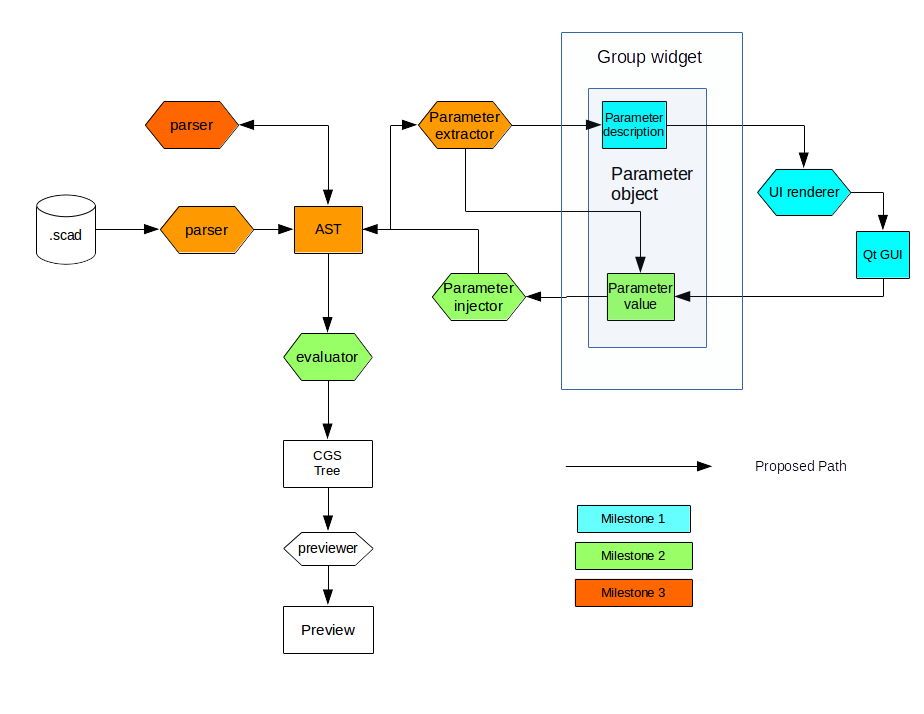
\includegraphics[width=\linewidth]{images/flowchart.png}
		\caption{Flowchart of Customizer}
		\label{fig:FD1}
	\end{figure}
	
	\item \textbf{Back End}
	This will include the parser part that will create AST nodes and we can extract the parameters from the AST. we can use the single parser for the whole .scad file or separate parser for extracting the parameters with annotations.
	The Back-end part will also include the parameter extractor and injector or the injector can be included in parameter object which will serve as interface
	\item \textbf{Interface}
	This will include the parameter object which will serve as an interface between both Back end and Front end. Parameter object will contain information regarding each individual parameter like parameter name, default value, and information how this parameter will be displayed as widgets to the user. Parameter object could also include the method to inject the value of the individual parameter into the AST.
	
\end{enumerate}

Implementation of the project will start with:
\begin{enumerate}
	\item Implementation of back End which will include defining the node for storing the annotation in AST and then linking it to rest of the AST. Then defining the parser for the parameters which will be feed with the text from the comment class which will act as link between the comment parser and main parser and it will also help in parsing the context sensitive grammar of the parameter which cannot be parsed by just using the flex and bison.
	\item After that the work on Interface will be started which include writing class ParameterObject which will contain the information about the Parameter Widget that has to be created and then ParameterExtractor class which will be used to extract and inject parameters into the AST.
	\item In Last, The GUI of the project will be defined which will include main ParameterWidget class to generate whole Customizer and parameterWidgetVirtual class which will be the base class for all the Parameter Widget. In Last, We will define groupWidget which will make groups of parameters and the ParameterSet class which will be used to define the Set of Parameter.
\end{enumerate}
 
\chapter{FACILITIES REQUIRED FOR PROPOSED WORK}

\section{Software Requirements}
The following softwares may be used while developing and testing the software:
\begin{enumerate} 
	\item A C++ compiler supporting C++11
	
	\item Qt$  4.4 \rightarrow 5.x $ (http://qt.io/ )
	
	\item QScintilla2 $ (2.7 \rightarrow $)(http://www.riverbankcomputing.co.uk/software/qscintilla/)
	
	\item CGAL ($ 3.6 \rightarrow $) (http://www.cgal.org/)
	
	\item GMP (5.x) (http://www.gmplib.org/)
	
	\item MPFR (3.x)(http://www.mpfr.org/)
	
	\item cmake ($ 2.8 \rightarrow $, required by CGAL and the test framework))(http://www.cmake.org/)
	
	\item boost ($ 1.35 \rightarrow $) (http://www.boost.org/)
	
	\item OpenCSG ($ 1.3.2 \rightarrow $)(http://www.opencsg.org/)
	
	\item GLEW ($ 1.5.4 \rightarrow $)(http://glew.sourceforge.net/)
	
	\item Eigen (3.x)(http://eigen.tuxfamily.org/)
	
	\item glib2 (2.x)(https://developer.gnome.org/glib/)
	
	\item fontconfig ($ 2.10 \rightarrow  $)(http://fontconfig.org/)
	
	\item freetype2 ($ 2.4 \rightarrow  $)(http://freetype.org/)
	
	\item harfbuzz ($ 0.9.19 \rightarrow  $)(http://harfbuzz.org/)
	
	\item Bison ($ 2.4 \rightarrow $ )(http://www.gnu.org/software/bison/)
	
	\item Flex ($ 2.5.35 \rightarrow  $)(http://flex.sourceforge.net/)
	
	\item pkg-config ($ 0.26 \rightarrow $ )(http://www.freedesktop.org/wiki/Software/pkg-config/)
	
\end{enumerate}

\addcontentsline{toc}{chapter}{BIBLIOGRAPHY}
\bibliographystyle{ieeetr} 
\begin{thebibliography}{22}

\bibitem{} "User:Amarjeet Singh Kapoor/GSoC2016/Project - BRL-CAD", Brlcad.org, 2016. [Online]. Available: http://brlcad.org/wiki/User:Amarjeet\_Singh\_Kapoor/GSoC2016/Project. [Accessed: 27- Nov- 2016].

\bibitem{} "OpenSCAD - News", Openscad.org, 2016. [Online]. Available: http://www.openscad.org/news.html\#20160714. [Accessed: 27- Nov- 2016].

\bibitem{} "OpenSCAD - News", Openscad.org, 2016. [Online]. Available: http://www.openscad.org/news.html\#20160714. [Accessed: 27- Nov- 2016].


\bibitem{} "openscad/openscad", GitHub, 2016. [Online]. Available: https://github.com/openscad/openscad. [Accessed: 27- Nov- 2016].

\bibitem{} "openscad/openscad", GitHub, 2016. [Online]. Available: https://github.com/openscad/openscad/wiki/Project\%3A-Form-based-script-parameterization. [Accessed: 27- Nov- 2016].

\bibitem{} "OpenSCAD", En.wikipedia.org, 2016. [Online]. Available: https://en.wikipedia.org/wiki/OpenSCAD. [Accessed: 27- Nov- 2016].

\end{thebibliography}
\end{document}

